\documentclass[a4paper,10pt,twoside]{article}

\usepackage[top=1in, bottom=1in, left=1in, right=1in]{geometry}
\usepackage[utf8]{inputenc}
\usepackage[spanish,es-ucroman,es-noquoting]{babel}
\usepackage{setspace}
\usepackage{fancyhdr}
\usepackage{lastpage}
\usepackage{amsmath}
\usepackage{amsfonts}
\usepackage{verbatim}
\usepackage{graphicx}
\usepackage{float}
\usepackage{algpseudocode}
\usepackage{enumitem} % Provee macro \setlist
\usepackage[toc, page]{appendix}


%%%%%%%%%% Configuración de Fancyhdr - Inicio %%%%%%%%%%
\pagestyle{fancy}
\thispagestyle{fancy}
\lhead{Trabajo Práctico 1 · Sistemas Operativos}
\rhead{Delgado · Lovisolo · Petaccio}
\renewcommand{\footrulewidth}{0.4pt}
\cfoot{\thepage /\pageref{LastPage}}

\fancypagestyle{caratula} {
   \fancyhf{}
   \cfoot{\thepage /\pageref{LastPage}}
   \renewcommand{\headrulewidth}{0pt}
   \renewcommand{\footrulewidth}{0pt}
}
%%%%%%%%%% Configuración de Fancyhdr - Fin %%%%%%%%%%


%%%%%%%%%% Configuración de Algorithmic - Inicio %%%%%%%%%%
% Entorno propio para customizar la presentación del pseudocódigo
\newenvironment{pseudo}[1][]{%
    \vspace{0.5em}%
    \begin{algorithmic}%
}
{%
    \end{algorithmic}%
    \vspace{0.5em}%
}

% Conectivo 'in' para usar así: \ForAll{$foo$ \In $bar$}
\newcommand{\In}{\textbf{in} }

% Conectivo 'to' para usar así: \For{$i = 1$ \In $n$}
\newcommand{\To}{\textbf{to} }

% Complejidades
\newcommand{\Ode}[1]{\hfill $O(#1)$}
%%%%%%%%%% Configuración de Algorithmic - Fin %%%%%%%%%%


%%%%%%%%%% Configuración de Appendix - Inicio %%%%%%%%%%
% Asigna la traducción de la palabra 'Appendices'.
\renewcommand{\appendixtocname}{Apéndices}
\renewcommand{\appendixpagename}{Apéndices}
%%%%%%%%%% Configuración de Appendix - Fin %%%%%%%%%%


%%%%%%%%%% Miscelánea - Inicio %%%%%%%%%%
% Evita que el documento se estire verticalmente para ocupar el espacio vacío
% en cada página.
\raggedbottom

% Deshabilita sangría en la primer línea de un párrafo.
\setlength{\parindent}{0em}

% Separación entre párrafos.
\setlength{\parskip}{0.5em}

% Separación entre elementos de listas.
\setlist{itemsep=0.5em}
%%%%%%%%%% Miscelánea - Fin %%%%%%%%%%


\begin{document}


%%%%%%%%%%%%%%%%%%%%%%%%%%%%%%%%%%%%%%%%%%%%%%%%%%%%%%%%%%%%%%%%%%%%%%%%%%%%%%%
%% Carátula                                                                  %%
%%%%%%%%%%%%%%%%%%%%%%%%%%%%%%%%%%%%%%%%%%%%%%%%%%%%%%%%%%%%%%%%%%%%%%%%%%%%%%%


\thispagestyle{caratula}

\begin{center}


\includegraphics[height=2cm]{DC.png} 
\hfill

\includegraphics[height=2cm]{UBA.jpg} 

\vspace{2cm}

Departamento de Computación,\\
Facultad de Ciencias Exactas y Naturales,\\
Universidad de Buenos Aires

\vspace{4cm}

\begin{Huge}
Trabajo Práctico 1
\end{Huge}

\vspace{0.5cm}

\begin{Large}
Sistemas Operativos
\end{Large}

\vspace{1cm}

Segundo Cuatrimestre de 2013

\vspace{4cm}

\begin{tabular}{|c|c|c|}
\hline
Apellido y Nombre & LU & E-mail\\
\hline
Alejandro Nahuel Delgado & 601/11 & nahueldelgado@gmail.com\\
Leandro Lovisolo      & 645/11 & leandro@leandro.me\\
Lautaro José Petaccio & 443/11 & lausuper@gmail.com\\
\hline
\end{tabular}

\end{center}

\newpage


%%%%%%%%%%%%%%%%%%%%%%%%%%%%%%%%%%%%%%%%%%%%%%%%%%%%%%%%%%%%%%%%%%%%%%%%%%%%%%%
%% Índice                                                                    %%
%%%%%%%%%%%%%%%%%%%%%%%%%%%%%%%%%%%%%%%%%%%%%%%%%%%%%%%%%%%%%%%%%%%%%%%%%%%%%%%


\tableofcontents

\newpage


%%%%%%%%%%%%%%%%%%%%%%%%%%%%%%%%%%%%%%%%%%%%%%%%%%%%%%%%%%%%%%%%%%%%%%%%%%%%%%%
%% Introducción                                                              %%
%%%%%%%%%%%%%%%%%%%%%%%%%%%%%%%%%%%%%%%%%%%%%%%%%%%%%%%%%%%%%%%%%%%%%%%%%%%%%%%


\section{Introducción}

Pendiente.


%%%%%%%%%%%%%%%%%%%%%%%%%%%%%%%%%%%%%%%%%%%%%%%%%%%%%%%%%%%%%%%%%%%%%%%%%%%%%%%
%% Ejercicio 1                                                               %%
%%%%%%%%%%%%%%%%%%%%%%%%%%%%%%%%%%%%%%%%%%%%%%%%%%%%%%%%%%%%%%%%%%%%%%%%%%%%%%%


\section{Ejercicio 1}

Pendiente.


%%%%%%%%%%%%%%%%%%%%%%%%%%%%%%%%%%%%%%%%%%%%%%%%%%%%%%%%%%%%%%%%%%%%%%%%%%%%%%%
%% Ejercicio 2                                                               %%
%%%%%%%%%%%%%%%%%%%%%%%%%%%%%%%%%%%%%%%%%%%%%%%%%%%%%%%%%%%%%%%%%%%%%%%%%%%%%%%


\section{Ejercicio 2}
El lote de tareas utilizado para el ejercicio es el siguiente:
\begin{pseudo}
	\State @0:
	\State TaskCPU 1000
	\State TaskConsola 3 100 200
	\State TaskConsola 5 150 270
\end{pseudo}

\begin{figure}[ht!]
\centering
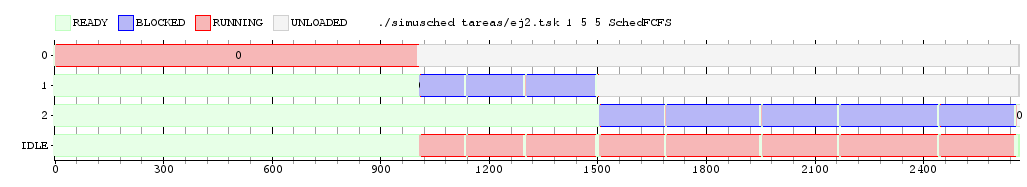
\includegraphics[width=175mm]{../ejercicio2/FCFS1Core.png}
\caption{Scheduler FCFS corriendo el lote de tareas con 1 core y 5 de penalidad por task switch}
\label{overflow}
\end{figure}

Puede observarse como el único core del scheduler para esta ejecución del simulador corre la tarea 0 hasta que esta se termina (1000 ticks).

Luego corre la tarea 1, la cuál realiza varios bloqueos y desbloqueos. Se puede notar el tiempo dedicado a hacer el task switch entre la tarea IDLE que corre mientras la tarea principal está bloqueada y la tarea principal.

Termina su ejecución con la tarea 2 que también realiza bloqueos y desbloqueos, intercambiando entre esta y su tarea IDLE.

\begin{figure}[ht!]
\centering
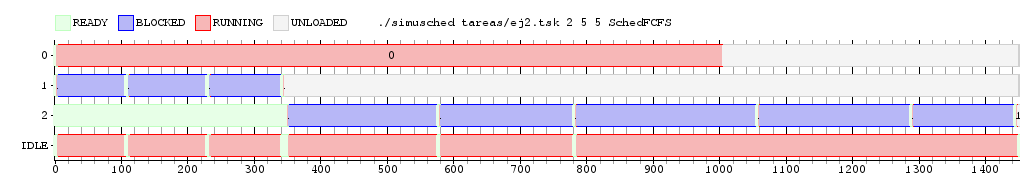
\includegraphics[width=175mm]{../ejercicio2/FCFS2Core.png}
\caption{Scheduler FCFS corriendo el lote de tareas con 2 core y 5 de penalidad por task switch}
\label{overflow}
\end{figure}

Puede observarse como en la figura 2, relacionada a la ejecución del simulador con 2 núcleos, como cada uno se comporta adecuadamente, tomando el core 0 la tarea 0, el core 1 la tarea 1 y ejecutándola hasta su finalización. Luego, como la tarea 1 finaliza antes que la 0, el core 0 toma la tarea 2 y la ejecuta.

\begin{figure}[ht!]
\centering
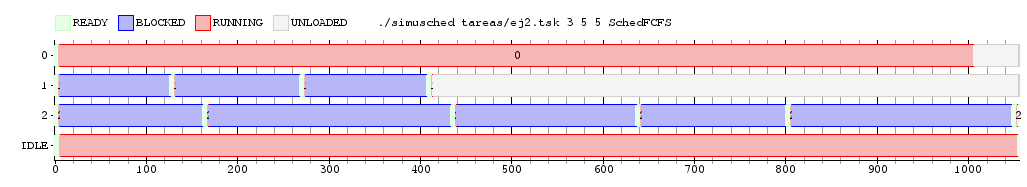
\includegraphics[width=175mm]{../ejercicio2/FCFS3Core.png}
\caption{Scheduler FCFS corriendo el lote de tareas con 3 core y 5 de penalidad por task switch}
\label{overflow}
\end{figure}

Observando la figura 3, puede notarse como cáda core toma cada una de las 3 tareas y las ejecuta simultáneamente hasta su finalización.

%%%%%%%%%%%%%%%%%%%%%%%%%%%%%%%%%%%%%%%%%%%%%%%%%%%%%%%%%%%%%%%%%%%%%%%%%%%%%%%
%% Ejercicio 3                                                               %%
%%%%%%%%%%%%%%%%%%%%%%%%%%%%%%%%%%%%%%%%%%%%%%%%%%%%%%%%%%%%%%%%%%%%%%%%%%%%%%%


\section{Ejercicio 3}

Pendiente.


%%%%%%%%%%%%%%%%%%%%%%%%%%%%%%%%%%%%%%%%%%%%%%%%%%%%%%%%%%%%%%%%%%%%%%%%%%%%%%%
%% Ejercicio 4                                                               %%
%%%%%%%%%%%%%%%%%%%%%%%%%%%%%%%%%%%%%%%%%%%%%%%%%%%%%%%%%%%%%%%%%%%%%%%%%%%%%%%


\section{Ejercicio 4}
El lote de tareas utilizado para la figura 4 es el siguiente:
\begin{pseudo}
	\State @0:
	\State TaskCPU 200
	\State TaskCPU 200
	\State TaskCPU 200
	\State TaskCPU 200
\end{pseudo}

Puede observarse en la figura 4 la ejecución del simulador con el Scheduler RoundRobin con 1 core con quantum 100 y penalidad de 5 para las task switch.

El gráfico muestra como las 4 tareas se ejecutan de forma cíclica, se ejecuta la tarea 0 a la 3 (haciendo cambio de tareas debido a que se les acaba el quantum) y se repite nuevamente este ciclo. Este comportamiento cíclcio de ejecución es el correspondiente al de un algoritmo de scheduling RoundRobin.

\begin{figure}[ht!]
\centering
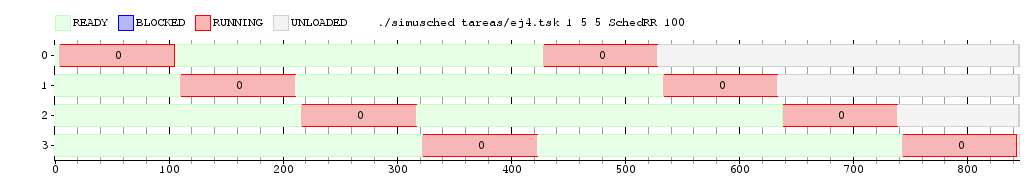
\includegraphics[width=175mm]{../ejercicio4/SchedRR1Core.png}
\caption{Scheduler RR corriendo el lote de tareas con 1 core con 100 de quantum y 5 de penalidad por task switch}
\label{overflow}
\end{figure}

El lote de tareas utilizado para la figura 5 es el siguiente:
\begin{pseudo}
	\State @0:
	\State TaskCPU 50
	\State TaskCPU 200
	\State TaskCPU 200
	\State TaskCPU 200
\end{pseudo}

Puede notarse nuevamente, en el gráfico de la figura 5, el cambio cíclico y ordenado de las tareas. En este caso, al tener una tarea de menor duración al inicio en el core 0, este queda asimétrico en relación al tiempo y a la ejecución de tareas, haciendo que en la próxima recorrida del ciclo del algoritmo, este tome las tareas del core 1, recibiendo una penalización de 50 ticks.

\begin{figure}[ht!]
\centering
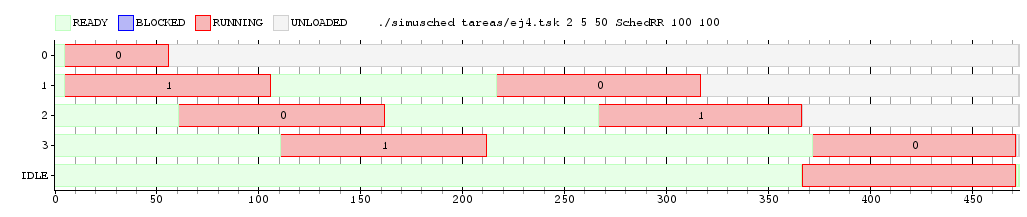
\includegraphics[width=175mm]{../ejercicio4/SchedRR2Core.png}
\caption{Scheduler RR corriendo el lote de tareas con 2 core de 100 de quantum cada uno y 50 de penalidad por task switch}
\label{overflow}
\end{figure}

El lote de tareas utilizado para la figura 6 es el siguiente:
\begin{pseudo}
	\State @0:
	\State TaskCPU 200
	\State TaskIO 50 400
	\State TaskCPU 200
	\State TaskCPU 200
\end{pseudo}

Por último, para demostrar la correctitud de la implementación del scheduler RoundRobin ante tareas bloqueantes, en la figura 6, puede verse como la tarea 1 se bloquea a los 50 ticks; el scheduler la remueve del ciclo continuando la ejecución las tareas sin tenerla en cuenta hasta que se realiza su desbloqueo, se agrega nuevamente al ciclo y termina.

\begin{figure}[ht!]
\centering
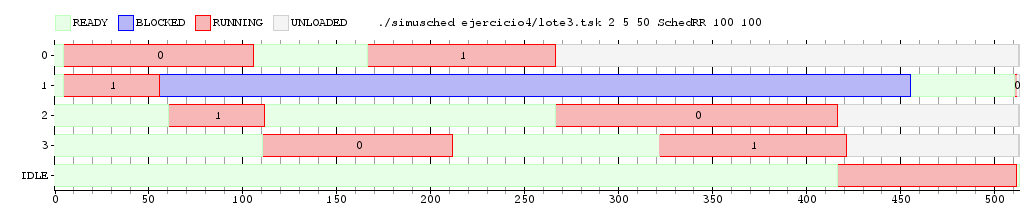
\includegraphics[width=175mm]{../ejercicio4/SchedRR2CoreIO.png}
\caption{Scheduler RR corriendo el lote de tareas con 2 core de 100 de quantum cada uno, 50 de penalidad por task switch y una tarea bloqueante}
\label{overflow}
\end{figure}

%%%%%%%%%%%%%%%%%%%%%%%%%%%%%%%%%%%%%%%%%%%%%%%%%%%%%%%%%%%%%%%%%%%%%%%%%%%%%%%
%% Ejercicio 5                                                               %%
%%%%%%%%%%%%%%%%%%%%%%%%%%%%%%%%%%%%%%%%%%%%%%%%%%%%%%%%%%%%%%%%%%%%%%%%%%%%%%%


\section{Ejercicio 5}

Pendiente.


%%%%%%%%%%%%%%%%%%%%%%%%%%%%%%%%%%%%%%%%%%%%%%%%%%%%%%%%%%%%%%%%%%%%%%%%%%%%%%%
%% Ejercicio 6                                                               %%
%%%%%%%%%%%%%%%%%%%%%%%%%%%%%%%%%%%%%%%%%%%%%%%%%%%%%%%%%%%%%%%%%%%%%%%%%%%%%%%


\section{Ejercicio 6}

Pendiente.


%%%%%%%%%%%%%%%%%%%%%%%%%%%%%%%%%%%%%%%%%%%%%%%%%%%%%%%%%%%%%%%%%%%%%%%%%%%%%%%
%% Ejercicio 7                                                               %%
%%%%%%%%%%%%%%%%%%%%%%%%%%%%%%%%%%%%%%%%%%%%%%%%%%%%%%%%%%%%%%%%%%%%%%%%%%%%%%%


\section{Ejercicio 7}

Diseñamos el siguiente lote de tareas:

\begin{verbatim}
*8 TaskBatch 8 1
*4 TaskBatch 8 2
*2 TaskBatch 8 4
TaskBatch 8 8
\end{verbatim}

Sobre el cual estudiamos las métricas a continuación:

\begin{description}
	\item[Tiempo de ejecución]
	Cantidad de ticks necesarios para completar todo el lote de tareas. Es el tiempo total que percibe el usuario desde que inicia el procesamiento de su lote de tareas hasta que éste termina.

	\item[Eficiencia]
	Relación entre los ciclos destinados a cómputos útiles y los ciclos totales utilizados hasta terminar de ejecutar el lote de tareas. Por cómputo útil se entiende un cómputo que forma parte de alguna de las tareas del lote, en lugar de uno que forma parte del scheduling (cambios de contexto, migraciones entre cores y tiempo idle).
\end{description}


\subsection{Experimentos}

Realizamos 4 experimentos para cada métrica: simulando 1, 2, 3 y 4 cores. Para cada experimento realizamos una simulación por cada una de las combinaciones de quantums posibles por core en el rango $1, \ldots, 8$.

Para los casos con 2 o más cores, recorremos el rango de quantums sin evaluar dos combinaciones equivalentes. \footnote{Por ejemplo, para el caso de 2 cores: las combinaciones de quantums $(5, 10)$ y $(10, 5)$ son equivalentes.} Esto lo logramos siguiendo las secuencias a continuación:

\begin{itemize}
	\item{
		Para 2 cores:
		$(1, 1), \ldots, (1, 8),
		 (2, 2), \ldots, (2, 8),
		 (3, 3), \ldots, (8, 8)$.
	}
	\item{
		Para 3 cores:
		$(1, 1, 1), \ldots, (1, 1, 8),
		 (1, 2, 2), \ldots, (1, 2, 8),
		 (1, 3, 3), \ldots, (8, 8, 8)$.
	}	
	\item{
		Para 4 cores:
		$(1, 1, 1, 1), \ldots, (1, 1, 1, 8),
		 (1, 1, 2, 2), \ldots, (1, 1, 8, 8),
		 (1, 2, 2, 2), \ldots, (1, 8, 8, 8)$, \\
		\hspace*{5.7em}
		$(2, 2, 2, 2), \ldots, (2, 8, 8, 8),
		 (3, 3, 3, 3), \ldots, (8, 8, 8, 8)$.
	}
\end{itemize}

En los resultados a continuación mostramos los valores mínimos y máximos observados para cada métrica.


\subsection{Tiempo de ejecución}


\subsubsection{1 core}

\begin{figure}[H]
	\centering
	% GNUPLOT: LaTeX picture with Postscript
\begingroup
  \makeatletter
  \providecommand\color[2][]{%
    \GenericError{(gnuplot) \space\space\space\@spaces}{%
      Package color not loaded in conjunction with
      terminal option `colourtext'%
    }{See the gnuplot documentation for explanation.%
    }{Either use 'blacktext' in gnuplot or load the package
      color.sty in LaTeX.}%
    \renewcommand\color[2][]{}%
  }%
  \providecommand\includegraphics[2][]{%
    \GenericError{(gnuplot) \space\space\space\@spaces}{%
      Package graphicx or graphics not loaded%
    }{See the gnuplot documentation for explanation.%
    }{The gnuplot epslatex terminal needs graphicx.sty or graphics.sty.}%
    \renewcommand\includegraphics[2][]{}%
  }%
  \providecommand\rotatebox[2]{#2}%
  \@ifundefined{ifGPcolor}{%
    \newif\ifGPcolor
    \GPcolorfalse
  }{}%
  \@ifundefined{ifGPblacktext}{%
    \newif\ifGPblacktext
    \GPblacktexttrue
  }{}%
  % define a \g@addto@macro without @ in the name:
  \let\gplgaddtomacro\g@addto@macro
  % define empty templates for all commands taking text:
  \gdef\gplbacktext{}%
  \gdef\gplfronttext{}%
  \makeatother
  \ifGPblacktext
    % no textcolor at all
    \def\colorrgb#1{}%
    \def\colorgray#1{}%
  \else
    % gray or color?
    \ifGPcolor
      \def\colorrgb#1{\color[rgb]{#1}}%
      \def\colorgray#1{\color[gray]{#1}}%
      \expandafter\def\csname LTw\endcsname{\color{white}}%
      \expandafter\def\csname LTb\endcsname{\color{black}}%
      \expandafter\def\csname LTa\endcsname{\color{black}}%
      \expandafter\def\csname LT0\endcsname{\color[rgb]{1,0,0}}%
      \expandafter\def\csname LT1\endcsname{\color[rgb]{0,1,0}}%
      \expandafter\def\csname LT2\endcsname{\color[rgb]{0,0,1}}%
      \expandafter\def\csname LT3\endcsname{\color[rgb]{1,0,1}}%
      \expandafter\def\csname LT4\endcsname{\color[rgb]{0,1,1}}%
      \expandafter\def\csname LT5\endcsname{\color[rgb]{1,1,0}}%
      \expandafter\def\csname LT6\endcsname{\color[rgb]{0,0,0}}%
      \expandafter\def\csname LT7\endcsname{\color[rgb]{1,0.3,0}}%
      \expandafter\def\csname LT8\endcsname{\color[rgb]{0.5,0.5,0.5}}%
    \else
      % gray
      \def\colorrgb#1{\color{black}}%
      \def\colorgray#1{\color[gray]{#1}}%
      \expandafter\def\csname LTw\endcsname{\color{white}}%
      \expandafter\def\csname LTb\endcsname{\color{black}}%
      \expandafter\def\csname LTa\endcsname{\color{black}}%
      \expandafter\def\csname LT0\endcsname{\color{black}}%
      \expandafter\def\csname LT1\endcsname{\color{black}}%
      \expandafter\def\csname LT2\endcsname{\color{black}}%
      \expandafter\def\csname LT3\endcsname{\color{black}}%
      \expandafter\def\csname LT4\endcsname{\color{black}}%
      \expandafter\def\csname LT5\endcsname{\color{black}}%
      \expandafter\def\csname LT6\endcsname{\color{black}}%
      \expandafter\def\csname LT7\endcsname{\color{black}}%
      \expandafter\def\csname LT8\endcsname{\color{black}}%
    \fi
  \fi
  \setlength{\unitlength}{0.0500bp}%
  \begin{picture}(9118.00,4320.00)%
    \gplgaddtomacro\gplbacktext{%
      \colorrgb{0.00,0.00,0.00}%
      \put(740,640){\makebox(0,0)[r]{\strut{}200}}%
      \colorrgb{0.00,0.00,0.00}%
      \put(740,1328){\makebox(0,0)[r]{\strut{}210}}%
      \colorrgb{0.00,0.00,0.00}%
      \put(740,2016){\makebox(0,0)[r]{\strut{}220}}%
      \colorrgb{0.00,0.00,0.00}%
      \put(740,2703){\makebox(0,0)[r]{\strut{}230}}%
      \colorrgb{0.00,0.00,0.00}%
      \put(740,3391){\makebox(0,0)[r]{\strut{}240}}%
      \colorrgb{0.00,0.00,0.00}%
      \put(740,4079){\makebox(0,0)[r]{\strut{}250}}%
      \colorrgb{0.00,0.00,0.00}%
      \put(860,440){\makebox(0,0){\strut{}$(1)$}}%
      \colorrgb{0.00,0.00,0.00}%
      \put(1988,440){\makebox(0,0){\strut{}$(2)$}}%
      \colorrgb{0.00,0.00,0.00}%
      \put(3116,440){\makebox(0,0){\strut{}$(3)$}}%
      \colorrgb{0.00,0.00,0.00}%
      \put(4244,440){\makebox(0,0){\strut{}$(4)$}}%
      \colorrgb{0.00,0.00,0.00}%
      \put(5373,440){\makebox(0,0){\strut{}$(5)$}}%
      \colorrgb{0.00,0.00,0.00}%
      \put(6501,440){\makebox(0,0){\strut{}$(6)$}}%
      \colorrgb{0.00,0.00,0.00}%
      \put(7629,440){\makebox(0,0){\strut{}$(7)$}}%
      \colorrgb{0.00,0.00,0.00}%
      \put(8757,440){\makebox(0,0){\strut{}$(8)$}}%
      \colorrgb{0.00,0.00,0.00}%
      \put(160,2359){\rotatebox{90}{\makebox(0,0){\strut{}Tiempo de ejecuci\'on (ticks)}}}%
      \colorrgb{0.00,0.00,0.00}%
      \put(4808,140){\makebox(0,0){\strut{}Quantums por core}}%
    }%
    \gplgaddtomacro\gplfronttext{%
      \csname LTb\endcsname%
      \put(7854,3916){\makebox(0,0)[r]{\strut{}M\'inimo}}%
      \csname LTb\endcsname%
      \put(7854,3716){\makebox(0,0)[r]{\strut{}M\'aximo}}%
    }%
    \gplbacktext
    \put(0,0){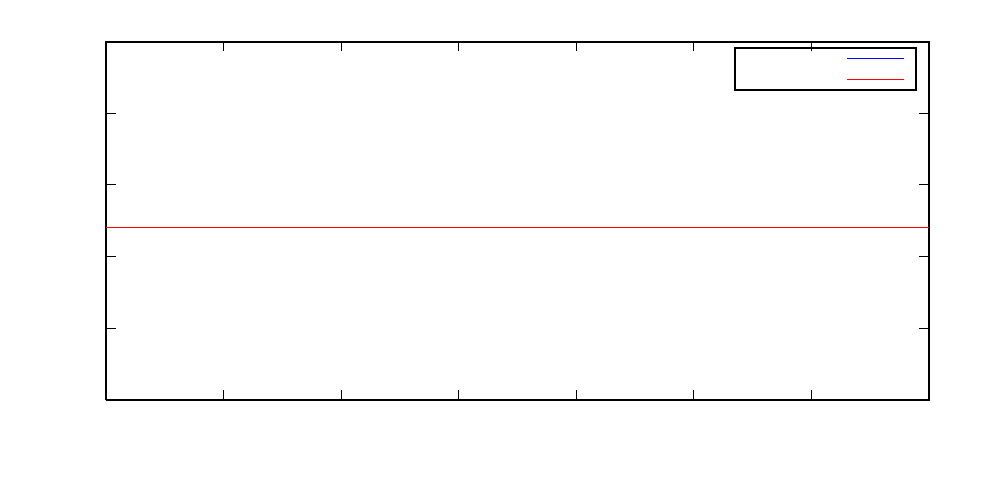
\includegraphics{ej7-grafico-runtime-1-core}}%
    \gplfronttext
  \end{picture}%
\endgroup

	\caption{Tiempo de ejecución en 1 core}
\end{figure}


\subsubsection{2 cores}

\begin{figure}[H]
	\centering
	% GNUPLOT: LaTeX picture with Postscript
\begingroup
  \makeatletter
  \providecommand\color[2][]{%
    \GenericError{(gnuplot) \space\space\space\@spaces}{%
      Package color not loaded in conjunction with
      terminal option `colourtext'%
    }{See the gnuplot documentation for explanation.%
    }{Either use 'blacktext' in gnuplot or load the package
      color.sty in LaTeX.}%
    \renewcommand\color[2][]{}%
  }%
  \providecommand\includegraphics[2][]{%
    \GenericError{(gnuplot) \space\space\space\@spaces}{%
      Package graphicx or graphics not loaded%
    }{See the gnuplot documentation for explanation.%
    }{The gnuplot epslatex terminal needs graphicx.sty or graphics.sty.}%
    \renewcommand\includegraphics[2][]{}%
  }%
  \providecommand\rotatebox[2]{#2}%
  \@ifundefined{ifGPcolor}{%
    \newif\ifGPcolor
    \GPcolorfalse
  }{}%
  \@ifundefined{ifGPblacktext}{%
    \newif\ifGPblacktext
    \GPblacktexttrue
  }{}%
  % define a \g@addto@macro without @ in the name:
  \let\gplgaddtomacro\g@addto@macro
  % define empty templates for all commands taking text:
  \gdef\gplbacktext{}%
  \gdef\gplfronttext{}%
  \makeatother
  \ifGPblacktext
    % no textcolor at all
    \def\colorrgb#1{}%
    \def\colorgray#1{}%
  \else
    % gray or color?
    \ifGPcolor
      \def\colorrgb#1{\color[rgb]{#1}}%
      \def\colorgray#1{\color[gray]{#1}}%
      \expandafter\def\csname LTw\endcsname{\color{white}}%
      \expandafter\def\csname LTb\endcsname{\color{black}}%
      \expandafter\def\csname LTa\endcsname{\color{black}}%
      \expandafter\def\csname LT0\endcsname{\color[rgb]{1,0,0}}%
      \expandafter\def\csname LT1\endcsname{\color[rgb]{0,1,0}}%
      \expandafter\def\csname LT2\endcsname{\color[rgb]{0,0,1}}%
      \expandafter\def\csname LT3\endcsname{\color[rgb]{1,0,1}}%
      \expandafter\def\csname LT4\endcsname{\color[rgb]{0,1,1}}%
      \expandafter\def\csname LT5\endcsname{\color[rgb]{1,1,0}}%
      \expandafter\def\csname LT6\endcsname{\color[rgb]{0,0,0}}%
      \expandafter\def\csname LT7\endcsname{\color[rgb]{1,0.3,0}}%
      \expandafter\def\csname LT8\endcsname{\color[rgb]{0.5,0.5,0.5}}%
    \else
      % gray
      \def\colorrgb#1{\color{black}}%
      \def\colorgray#1{\color[gray]{#1}}%
      \expandafter\def\csname LTw\endcsname{\color{white}}%
      \expandafter\def\csname LTb\endcsname{\color{black}}%
      \expandafter\def\csname LTa\endcsname{\color{black}}%
      \expandafter\def\csname LT0\endcsname{\color{black}}%
      \expandafter\def\csname LT1\endcsname{\color{black}}%
      \expandafter\def\csname LT2\endcsname{\color{black}}%
      \expandafter\def\csname LT3\endcsname{\color{black}}%
      \expandafter\def\csname LT4\endcsname{\color{black}}%
      \expandafter\def\csname LT5\endcsname{\color{black}}%
      \expandafter\def\csname LT6\endcsname{\color{black}}%
      \expandafter\def\csname LT7\endcsname{\color{black}}%
      \expandafter\def\csname LT8\endcsname{\color{black}}%
    \fi
  \fi
  \setlength{\unitlength}{0.0500bp}%
  \begin{picture}(9118.00,4320.00)%
    \gplgaddtomacro\gplbacktext{%
      \colorrgb{0.00,0.00,0.00}%
      \put(740,640){\makebox(0,0)[r]{\strut{}125}}%
      \colorrgb{0.00,0.00,0.00}%
      \put(740,1131){\makebox(0,0)[r]{\strut{}130}}%
      \colorrgb{0.00,0.00,0.00}%
      \put(740,1623){\makebox(0,0)[r]{\strut{}135}}%
      \colorrgb{0.00,0.00,0.00}%
      \put(740,2114){\makebox(0,0)[r]{\strut{}140}}%
      \colorrgb{0.00,0.00,0.00}%
      \put(740,2605){\makebox(0,0)[r]{\strut{}145}}%
      \colorrgb{0.00,0.00,0.00}%
      \put(740,3096){\makebox(0,0)[r]{\strut{}150}}%
      \colorrgb{0.00,0.00,0.00}%
      \put(740,3588){\makebox(0,0)[r]{\strut{}155}}%
      \colorrgb{0.00,0.00,0.00}%
      \put(740,4079){\makebox(0,0)[r]{\strut{}160}}%
      \colorrgb{0.00,0.00,0.00}%
      \put(860,440){\makebox(0,0){\strut{}$(1, *)$}}%
      \colorrgb{0.00,0.00,0.00}%
      \put(1971,440){\makebox(0,0){\strut{}$(2, *)$}}%
      \colorrgb{0.00,0.00,0.00}%
      \put(3082,440){\makebox(0,0){\strut{}$(3, *)$}}%
      \colorrgb{0.00,0.00,0.00}%
      \put(4193,440){\makebox(0,0){\strut{}$(4, *)$}}%
      \colorrgb{0.00,0.00,0.00}%
      \put(5305,440){\makebox(0,0){\strut{}$(5, *)$}}%
      \colorrgb{0.00,0.00,0.00}%
      \put(6416,440){\makebox(0,0){\strut{}$(6, *)$}}%
      \colorrgb{0.00,0.00,0.00}%
      \put(7527,440){\makebox(0,0){\strut{}$(7, *)$}}%
      \colorrgb{0.00,0.00,0.00}%
      \put(8638,440){\makebox(0,0){\strut{}$(8, *)$}}%
      \colorrgb{0.00,0.00,0.00}%
      \put(160,2359){\rotatebox{90}{\makebox(0,0){\strut{}Tiempo de ejecuci\'on (ticks)}}}%
      \colorrgb{0.00,0.00,0.00}%
      \put(4749,140){\makebox(0,0){\strut{}Quantums por core}}%
    }%
    \gplgaddtomacro\gplfronttext{%
      \csname LTb\endcsname%
      \put(7735,3916){\makebox(0,0)[r]{\strut{}M\'inimo}}%
      \csname LTb\endcsname%
      \put(7735,3716){\makebox(0,0)[r]{\strut{}M\'aximo}}%
    }%
    \gplbacktext
    \put(0,0){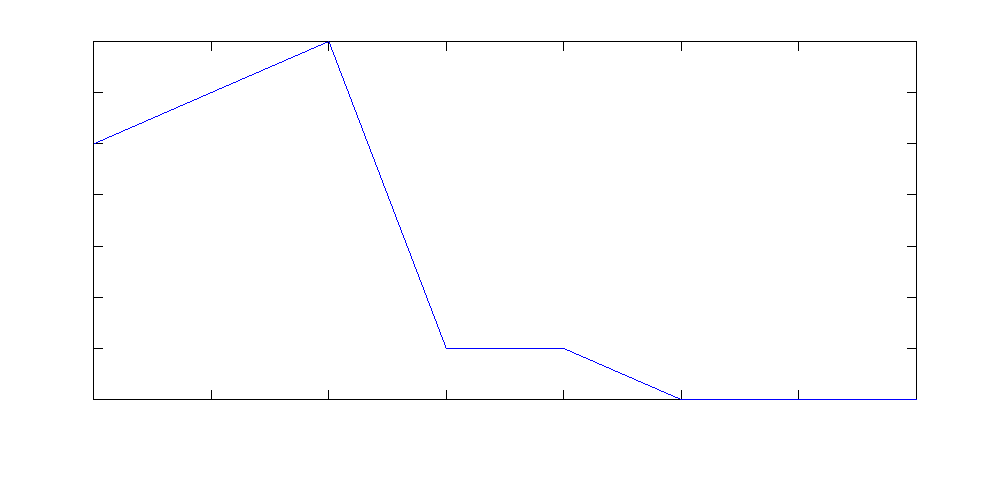
\includegraphics{ej7-grafico-runtime-2-cores}}%
    \gplfronttext
  \end{picture}%
\endgroup

	\caption{Tiempo de ejecución en 2 cores}
\end{figure}


\subsubsection{3 cores}

\begin{figure}[H]
	\centering
	% GNUPLOT: LaTeX picture with Postscript
\begingroup
  \makeatletter
  \providecommand\color[2][]{%
    \GenericError{(gnuplot) \space\space\space\@spaces}{%
      Package color not loaded in conjunction with
      terminal option `colourtext'%
    }{See the gnuplot documentation for explanation.%
    }{Either use 'blacktext' in gnuplot or load the package
      color.sty in LaTeX.}%
    \renewcommand\color[2][]{}%
  }%
  \providecommand\includegraphics[2][]{%
    \GenericError{(gnuplot) \space\space\space\@spaces}{%
      Package graphicx or graphics not loaded%
    }{See the gnuplot documentation for explanation.%
    }{The gnuplot epslatex terminal needs graphicx.sty or graphics.sty.}%
    \renewcommand\includegraphics[2][]{}%
  }%
  \providecommand\rotatebox[2]{#2}%
  \@ifundefined{ifGPcolor}{%
    \newif\ifGPcolor
    \GPcolorfalse
  }{}%
  \@ifundefined{ifGPblacktext}{%
    \newif\ifGPblacktext
    \GPblacktexttrue
  }{}%
  % define a \g@addto@macro without @ in the name:
  \let\gplgaddtomacro\g@addto@macro
  % define empty templates for all commands taking text:
  \gdef\gplbacktext{}%
  \gdef\gplfronttext{}%
  \makeatother
  \ifGPblacktext
    % no textcolor at all
    \def\colorrgb#1{}%
    \def\colorgray#1{}%
  \else
    % gray or color?
    \ifGPcolor
      \def\colorrgb#1{\color[rgb]{#1}}%
      \def\colorgray#1{\color[gray]{#1}}%
      \expandafter\def\csname LTw\endcsname{\color{white}}%
      \expandafter\def\csname LTb\endcsname{\color{black}}%
      \expandafter\def\csname LTa\endcsname{\color{black}}%
      \expandafter\def\csname LT0\endcsname{\color[rgb]{1,0,0}}%
      \expandafter\def\csname LT1\endcsname{\color[rgb]{0,1,0}}%
      \expandafter\def\csname LT2\endcsname{\color[rgb]{0,0,1}}%
      \expandafter\def\csname LT3\endcsname{\color[rgb]{1,0,1}}%
      \expandafter\def\csname LT4\endcsname{\color[rgb]{0,1,1}}%
      \expandafter\def\csname LT5\endcsname{\color[rgb]{1,1,0}}%
      \expandafter\def\csname LT6\endcsname{\color[rgb]{0,0,0}}%
      \expandafter\def\csname LT7\endcsname{\color[rgb]{1,0.3,0}}%
      \expandafter\def\csname LT8\endcsname{\color[rgb]{0.5,0.5,0.5}}%
    \else
      % gray
      \def\colorrgb#1{\color{black}}%
      \def\colorgray#1{\color[gray]{#1}}%
      \expandafter\def\csname LTw\endcsname{\color{white}}%
      \expandafter\def\csname LTb\endcsname{\color{black}}%
      \expandafter\def\csname LTa\endcsname{\color{black}}%
      \expandafter\def\csname LT0\endcsname{\color{black}}%
      \expandafter\def\csname LT1\endcsname{\color{black}}%
      \expandafter\def\csname LT2\endcsname{\color{black}}%
      \expandafter\def\csname LT3\endcsname{\color{black}}%
      \expandafter\def\csname LT4\endcsname{\color{black}}%
      \expandafter\def\csname LT5\endcsname{\color{black}}%
      \expandafter\def\csname LT6\endcsname{\color{black}}%
      \expandafter\def\csname LT7\endcsname{\color{black}}%
      \expandafter\def\csname LT8\endcsname{\color{black}}%
    \fi
  \fi
  \setlength{\unitlength}{0.0500bp}%
  \begin{picture}(9118.00,4320.00)%
    \gplgaddtomacro\gplbacktext{%
      \colorrgb{0.00,0.00,0.00}%
      \put(620,640){\makebox(0,0)[r]{\strut{}38}}%
      \colorrgb{0.00,0.00,0.00}%
      \put(620,1131){\makebox(0,0)[r]{\strut{}39}}%
      \colorrgb{0.00,0.00,0.00}%
      \put(620,1623){\makebox(0,0)[r]{\strut{}40}}%
      \colorrgb{0.00,0.00,0.00}%
      \put(620,2114){\makebox(0,0)[r]{\strut{}41}}%
      \colorrgb{0.00,0.00,0.00}%
      \put(620,2605){\makebox(0,0)[r]{\strut{}42}}%
      \colorrgb{0.00,0.00,0.00}%
      \put(620,3096){\makebox(0,0)[r]{\strut{}43}}%
      \colorrgb{0.00,0.00,0.00}%
      \put(620,3588){\makebox(0,0)[r]{\strut{}44}}%
      \colorrgb{0.00,0.00,0.00}%
      \put(620,4079){\makebox(0,0)[r]{\strut{}45}}%
      \colorrgb{0.00,0.00,0.00}%
      \put(740,440){\makebox(0,0){\strut{}$(1, *, *)$}}%
      \colorrgb{0.00,0.00,0.00}%
      \put(1843,440){\makebox(0,0){\strut{}$(2, *, *)$}}%
      \colorrgb{0.00,0.00,0.00}%
      \put(2945,440){\makebox(0,0){\strut{}$(3, *, *)$}}%
      \colorrgb{0.00,0.00,0.00}%
      \put(4048,440){\makebox(0,0){\strut{}$(4, *, *)$}}%
      \colorrgb{0.00,0.00,0.00}%
      \put(5150,440){\makebox(0,0){\strut{}$(5, *, *)$}}%
      \colorrgb{0.00,0.00,0.00}%
      \put(6253,440){\makebox(0,0){\strut{}$(6, *, *)$}}%
      \colorrgb{0.00,0.00,0.00}%
      \put(7355,440){\makebox(0,0){\strut{}$(7, *, *)$}}%
      \colorrgb{0.00,0.00,0.00}%
      \put(8458,440){\makebox(0,0){\strut{}$(8, *, *)$}}%
      \colorrgb{0.00,0.00,0.00}%
      \put(160,2359){\rotatebox{90}{\makebox(0,0){\strut{}Tiempo de ejecuci\'on (ticks)}}}%
      \colorrgb{0.00,0.00,0.00}%
      \put(4599,140){\makebox(0,0){\strut{}Quantums por core}}%
    }%
    \gplgaddtomacro\gplfronttext{%
      \csname LTb\endcsname%
      \put(7555,3916){\makebox(0,0)[r]{\strut{}M\'inimo}}%
      \csname LTb\endcsname%
      \put(7555,3716){\makebox(0,0)[r]{\strut{}M\'aximo}}%
    }%
    \gplbacktext
    \put(0,0){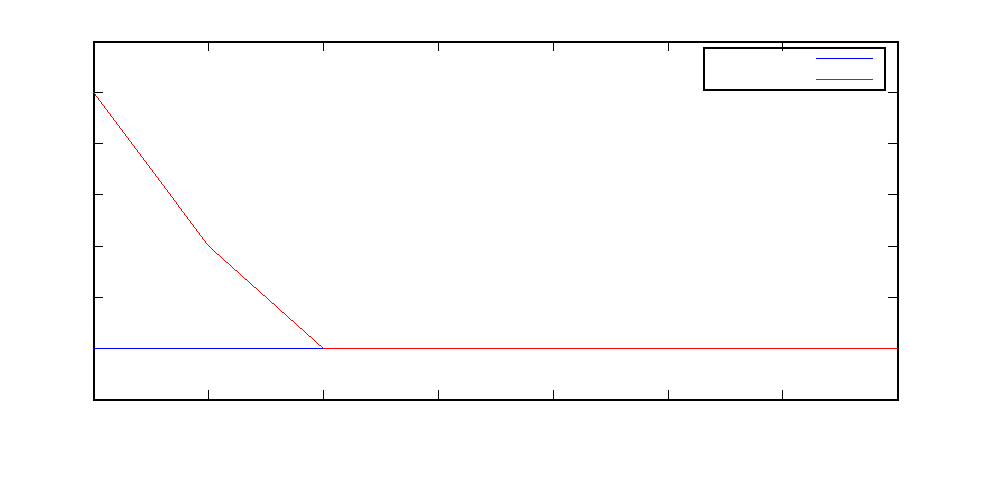
\includegraphics{ej7-grafico-runtime-3-cores}}%
    \gplfronttext
  \end{picture}%
\endgroup

	\caption{Tiempos de ejecución mínimos y máximos en 3 cores}
\end{figure}


\subsubsection{4 cores}

\begin{figure}[H]
	\centering
	% GNUPLOT: LaTeX picture with Postscript
\begingroup
  \makeatletter
  \providecommand\color[2][]{%
    \GenericError{(gnuplot) \space\space\space\@spaces}{%
      Package color not loaded in conjunction with
      terminal option `colourtext'%
    }{See the gnuplot documentation for explanation.%
    }{Either use 'blacktext' in gnuplot or load the package
      color.sty in LaTeX.}%
    \renewcommand\color[2][]{}%
  }%
  \providecommand\includegraphics[2][]{%
    \GenericError{(gnuplot) \space\space\space\@spaces}{%
      Package graphicx or graphics not loaded%
    }{See the gnuplot documentation for explanation.%
    }{The gnuplot epslatex terminal needs graphicx.sty or graphics.sty.}%
    \renewcommand\includegraphics[2][]{}%
  }%
  \providecommand\rotatebox[2]{#2}%
  \@ifundefined{ifGPcolor}{%
    \newif\ifGPcolor
    \GPcolorfalse
  }{}%
  \@ifundefined{ifGPblacktext}{%
    \newif\ifGPblacktext
    \GPblacktexttrue
  }{}%
  % define a \g@addto@macro without @ in the name:
  \let\gplgaddtomacro\g@addto@macro
  % define empty templates for all commands taking text:
  \gdef\gplbacktext{}%
  \gdef\gplfronttext{}%
  \makeatother
  \ifGPblacktext
    % no textcolor at all
    \def\colorrgb#1{}%
    \def\colorgray#1{}%
  \else
    % gray or color?
    \ifGPcolor
      \def\colorrgb#1{\color[rgb]{#1}}%
      \def\colorgray#1{\color[gray]{#1}}%
      \expandafter\def\csname LTw\endcsname{\color{white}}%
      \expandafter\def\csname LTb\endcsname{\color{black}}%
      \expandafter\def\csname LTa\endcsname{\color{black}}%
      \expandafter\def\csname LT0\endcsname{\color[rgb]{1,0,0}}%
      \expandafter\def\csname LT1\endcsname{\color[rgb]{0,1,0}}%
      \expandafter\def\csname LT2\endcsname{\color[rgb]{0,0,1}}%
      \expandafter\def\csname LT3\endcsname{\color[rgb]{1,0,1}}%
      \expandafter\def\csname LT4\endcsname{\color[rgb]{0,1,1}}%
      \expandafter\def\csname LT5\endcsname{\color[rgb]{1,1,0}}%
      \expandafter\def\csname LT6\endcsname{\color[rgb]{0,0,0}}%
      \expandafter\def\csname LT7\endcsname{\color[rgb]{1,0.3,0}}%
      \expandafter\def\csname LT8\endcsname{\color[rgb]{0.5,0.5,0.5}}%
    \else
      % gray
      \def\colorrgb#1{\color{black}}%
      \def\colorgray#1{\color[gray]{#1}}%
      \expandafter\def\csname LTw\endcsname{\color{white}}%
      \expandafter\def\csname LTb\endcsname{\color{black}}%
      \expandafter\def\csname LTa\endcsname{\color{black}}%
      \expandafter\def\csname LT0\endcsname{\color{black}}%
      \expandafter\def\csname LT1\endcsname{\color{black}}%
      \expandafter\def\csname LT2\endcsname{\color{black}}%
      \expandafter\def\csname LT3\endcsname{\color{black}}%
      \expandafter\def\csname LT4\endcsname{\color{black}}%
      \expandafter\def\csname LT5\endcsname{\color{black}}%
      \expandafter\def\csname LT6\endcsname{\color{black}}%
      \expandafter\def\csname LT7\endcsname{\color{black}}%
      \expandafter\def\csname LT8\endcsname{\color{black}}%
    \fi
  \fi
  \setlength{\unitlength}{0.0500bp}%
  \begin{picture}(9118.00,4320.00)%
    \gplgaddtomacro\gplbacktext{%
      \colorrgb{0.00,0.00,0.00}%
      \put(620,640){\makebox(0,0)[r]{\strut{}30}}%
      \colorrgb{0.00,0.00,0.00}%
      \put(620,1328){\makebox(0,0)[r]{\strut{}31}}%
      \colorrgb{0.00,0.00,0.00}%
      \put(620,2016){\makebox(0,0)[r]{\strut{}32}}%
      \colorrgb{0.00,0.00,0.00}%
      \put(620,2703){\makebox(0,0)[r]{\strut{}33}}%
      \colorrgb{0.00,0.00,0.00}%
      \put(620,3391){\makebox(0,0)[r]{\strut{}34}}%
      \colorrgb{0.00,0.00,0.00}%
      \put(620,4079){\makebox(0,0)[r]{\strut{}35}}%
      \colorrgb{0.00,0.00,0.00}%
      \put(740,440){\makebox(0,0){\strut{}$(1, *, *, *)$}}%
      \colorrgb{0.00,0.00,0.00}%
      \put(1817,440){\makebox(0,0){\strut{}$(2, *, *, *)$}}%
      \colorrgb{0.00,0.00,0.00}%
      \put(2894,440){\makebox(0,0){\strut{}$(3, *, *, *)$}}%
      \colorrgb{0.00,0.00,0.00}%
      \put(3971,440){\makebox(0,0){\strut{}$(4, *, *, *)$}}%
      \colorrgb{0.00,0.00,0.00}%
      \put(5047,440){\makebox(0,0){\strut{}$(5, *, *, *)$}}%
      \colorrgb{0.00,0.00,0.00}%
      \put(6124,440){\makebox(0,0){\strut{}$(6, *, *, *)$}}%
      \colorrgb{0.00,0.00,0.00}%
      \put(7201,440){\makebox(0,0){\strut{}$(7, *, *, *)$}}%
      \colorrgb{0.00,0.00,0.00}%
      \put(8278,440){\makebox(0,0){\strut{}$(8, *, *, *)$}}%
      \colorrgb{0.00,0.00,0.00}%
      \put(160,2359){\rotatebox{90}{\makebox(0,0){\strut{}Tiempo de ejecuci\'on (ticks)}}}%
      \colorrgb{0.00,0.00,0.00}%
      \put(4509,140){\makebox(0,0){\strut{}Quantums por core}}%
    }%
    \gplgaddtomacro\gplfronttext{%
      \csname LTb\endcsname%
      \put(7375,3916){\makebox(0,0)[r]{\strut{}M\'inimo}}%
      \csname LTb\endcsname%
      \put(7375,3716){\makebox(0,0)[r]{\strut{}M\'aximo}}%
    }%
    \gplbacktext
    \put(0,0){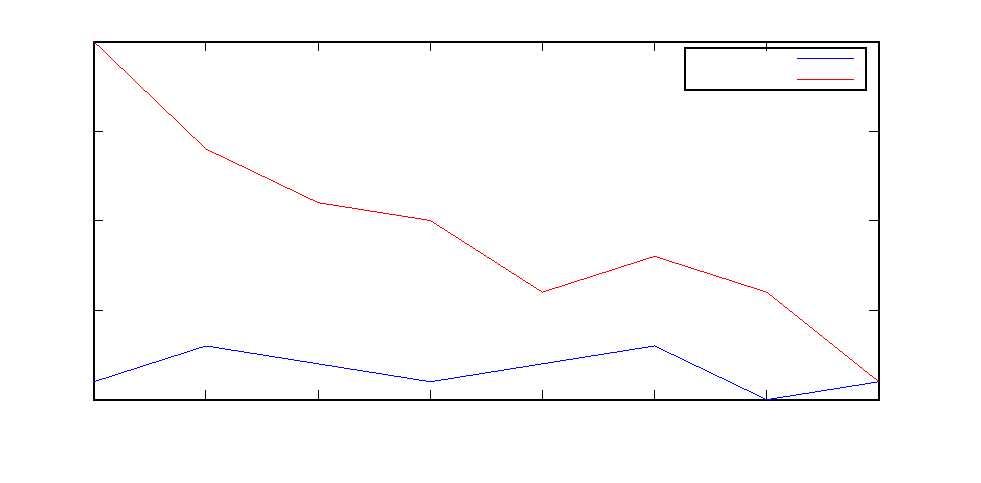
\includegraphics{ej7-grafico-runtime-4-cores}}%
    \gplfronttext
  \end{picture}%
\endgroup

	\caption{Tiempos de ejecución mínimos y máximos en 4 cores}
\end{figure}


\subsection{Eficiencia}


\subsubsection{1 core}

\begin{figure}[H]
	\centering
	% GNUPLOT: LaTeX picture with Postscript
\begingroup
  \makeatletter
  \providecommand\color[2][]{%
    \GenericError{(gnuplot) \space\space\space\@spaces}{%
      Package color not loaded in conjunction with
      terminal option `colourtext'%
    }{See the gnuplot documentation for explanation.%
    }{Either use 'blacktext' in gnuplot or load the package
      color.sty in LaTeX.}%
    \renewcommand\color[2][]{}%
  }%
  \providecommand\includegraphics[2][]{%
    \GenericError{(gnuplot) \space\space\space\@spaces}{%
      Package graphicx or graphics not loaded%
    }{See the gnuplot documentation for explanation.%
    }{The gnuplot epslatex terminal needs graphicx.sty or graphics.sty.}%
    \renewcommand\includegraphics[2][]{}%
  }%
  \providecommand\rotatebox[2]{#2}%
  \@ifundefined{ifGPcolor}{%
    \newif\ifGPcolor
    \GPcolorfalse
  }{}%
  \@ifundefined{ifGPblacktext}{%
    \newif\ifGPblacktext
    \GPblacktexttrue
  }{}%
  % define a \g@addto@macro without @ in the name:
  \let\gplgaddtomacro\g@addto@macro
  % define empty templates for all commands taking text:
  \gdef\gplbacktext{}%
  \gdef\gplfronttext{}%
  \makeatother
  \ifGPblacktext
    % no textcolor at all
    \def\colorrgb#1{}%
    \def\colorgray#1{}%
  \else
    % gray or color?
    \ifGPcolor
      \def\colorrgb#1{\color[rgb]{#1}}%
      \def\colorgray#1{\color[gray]{#1}}%
      \expandafter\def\csname LTw\endcsname{\color{white}}%
      \expandafter\def\csname LTb\endcsname{\color{black}}%
      \expandafter\def\csname LTa\endcsname{\color{black}}%
      \expandafter\def\csname LT0\endcsname{\color[rgb]{1,0,0}}%
      \expandafter\def\csname LT1\endcsname{\color[rgb]{0,1,0}}%
      \expandafter\def\csname LT2\endcsname{\color[rgb]{0,0,1}}%
      \expandafter\def\csname LT3\endcsname{\color[rgb]{1,0,1}}%
      \expandafter\def\csname LT4\endcsname{\color[rgb]{0,1,1}}%
      \expandafter\def\csname LT5\endcsname{\color[rgb]{1,1,0}}%
      \expandafter\def\csname LT6\endcsname{\color[rgb]{0,0,0}}%
      \expandafter\def\csname LT7\endcsname{\color[rgb]{1,0.3,0}}%
      \expandafter\def\csname LT8\endcsname{\color[rgb]{0.5,0.5,0.5}}%
    \else
      % gray
      \def\colorrgb#1{\color{black}}%
      \def\colorgray#1{\color[gray]{#1}}%
      \expandafter\def\csname LTw\endcsname{\color{white}}%
      \expandafter\def\csname LTb\endcsname{\color{black}}%
      \expandafter\def\csname LTa\endcsname{\color{black}}%
      \expandafter\def\csname LT0\endcsname{\color{black}}%
      \expandafter\def\csname LT1\endcsname{\color{black}}%
      \expandafter\def\csname LT2\endcsname{\color{black}}%
      \expandafter\def\csname LT3\endcsname{\color{black}}%
      \expandafter\def\csname LT4\endcsname{\color{black}}%
      \expandafter\def\csname LT5\endcsname{\color{black}}%
      \expandafter\def\csname LT6\endcsname{\color{black}}%
      \expandafter\def\csname LT7\endcsname{\color{black}}%
      \expandafter\def\csname LT8\endcsname{\color{black}}%
    \fi
  \fi
  \setlength{\unitlength}{0.0500bp}%
  \begin{picture}(9118.00,4320.00)%
    \gplgaddtomacro\gplbacktext{%
      \colorrgb{0.00,0.00,0.00}%
      \put(860,640){\makebox(0,0)[r]{\strut{}0.54}}%
      \colorrgb{0.00,0.00,0.00}%
      \put(860,1213){\makebox(0,0)[r]{\strut{}0.56}}%
      \colorrgb{0.00,0.00,0.00}%
      \put(860,1786){\makebox(0,0)[r]{\strut{}0.58}}%
      \colorrgb{0.00,0.00,0.00}%
      \put(860,2360){\makebox(0,0)[r]{\strut{}0.6}}%
      \colorrgb{0.00,0.00,0.00}%
      \put(860,2933){\makebox(0,0)[r]{\strut{}0.62}}%
      \colorrgb{0.00,0.00,0.00}%
      \put(860,3506){\makebox(0,0)[r]{\strut{}0.64}}%
      \colorrgb{0.00,0.00,0.00}%
      \put(860,4079){\makebox(0,0)[r]{\strut{}0.66}}%
      \colorrgb{0.00,0.00,0.00}%
      \put(980,440){\makebox(0,0){\strut{}$(1)$}}%
      \colorrgb{0.00,0.00,0.00}%
      \put(2091,440){\makebox(0,0){\strut{}$(2)$}}%
      \colorrgb{0.00,0.00,0.00}%
      \put(3202,440){\makebox(0,0){\strut{}$(3)$}}%
      \colorrgb{0.00,0.00,0.00}%
      \put(4313,440){\makebox(0,0){\strut{}$(4)$}}%
      \colorrgb{0.00,0.00,0.00}%
      \put(5424,440){\makebox(0,0){\strut{}$(5)$}}%
      \colorrgb{0.00,0.00,0.00}%
      \put(6535,440){\makebox(0,0){\strut{}$(6)$}}%
      \colorrgb{0.00,0.00,0.00}%
      \put(7646,440){\makebox(0,0){\strut{}$(7)$}}%
      \colorrgb{0.00,0.00,0.00}%
      \put(8757,440){\makebox(0,0){\strut{}$(8)$}}%
      \colorrgb{0.00,0.00,0.00}%
      \put(160,2359){\rotatebox{90}{\makebox(0,0){\strut{}Eficiencia (ciclos \'utiles / ciclos totales)}}}%
      \colorrgb{0.00,0.00,0.00}%
      \put(4868,140){\makebox(0,0){\strut{}Quantums por core}}%
    }%
    \gplgaddtomacro\gplfronttext{%
      \csname LTb\endcsname%
      \put(7854,3916){\makebox(0,0)[r]{\strut{}M\'inimo}}%
      \csname LTb\endcsname%
      \put(7854,3716){\makebox(0,0)[r]{\strut{}M\'aximo}}%
    }%
    \gplbacktext
    \put(0,0){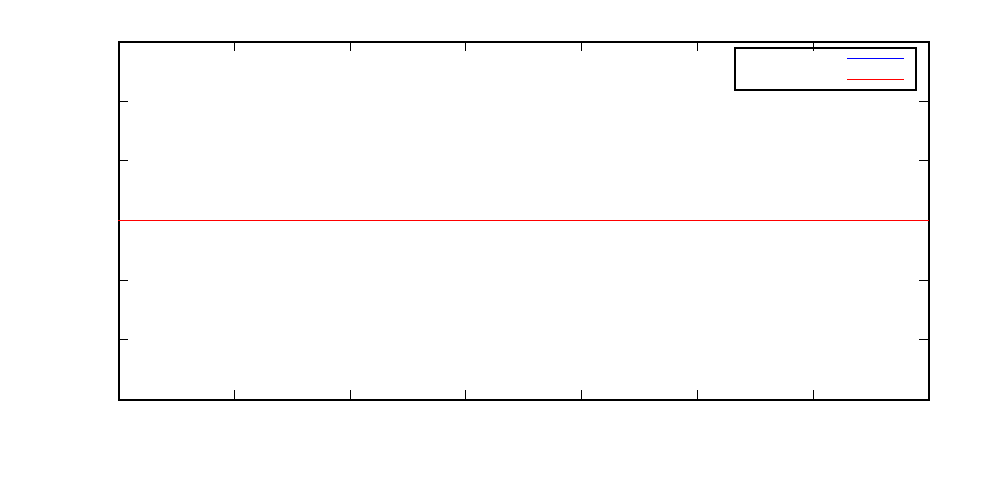
\includegraphics{ej7-grafico-eficiencia-1-core}}%
    \gplfronttext
  \end{picture}%
\endgroup

	\caption{Tiempos de ejecución mínimos y máximos en 1 core}
\end{figure}


\subsubsection{2 cores}

\begin{figure}[H]
	\centering
	% GNUPLOT: LaTeX picture with Postscript
\begingroup
  \makeatletter
  \providecommand\color[2][]{%
    \GenericError{(gnuplot) \space\space\space\@spaces}{%
      Package color not loaded in conjunction with
      terminal option `colourtext'%
    }{See the gnuplot documentation for explanation.%
    }{Either use 'blacktext' in gnuplot or load the package
      color.sty in LaTeX.}%
    \renewcommand\color[2][]{}%
  }%
  \providecommand\includegraphics[2][]{%
    \GenericError{(gnuplot) \space\space\space\@spaces}{%
      Package graphicx or graphics not loaded%
    }{See the gnuplot documentation for explanation.%
    }{The gnuplot epslatex terminal needs graphicx.sty or graphics.sty.}%
    \renewcommand\includegraphics[2][]{}%
  }%
  \providecommand\rotatebox[2]{#2}%
  \@ifundefined{ifGPcolor}{%
    \newif\ifGPcolor
    \GPcolorfalse
  }{}%
  \@ifundefined{ifGPblacktext}{%
    \newif\ifGPblacktext
    \GPblacktexttrue
  }{}%
  % define a \g@addto@macro without @ in the name:
  \let\gplgaddtomacro\g@addto@macro
  % define empty templates for all commands taking text:
  \gdef\gplbacktext{}%
  \gdef\gplfronttext{}%
  \makeatother
  \ifGPblacktext
    % no textcolor at all
    \def\colorrgb#1{}%
    \def\colorgray#1{}%
  \else
    % gray or color?
    \ifGPcolor
      \def\colorrgb#1{\color[rgb]{#1}}%
      \def\colorgray#1{\color[gray]{#1}}%
      \expandafter\def\csname LTw\endcsname{\color{white}}%
      \expandafter\def\csname LTb\endcsname{\color{black}}%
      \expandafter\def\csname LTa\endcsname{\color{black}}%
      \expandafter\def\csname LT0\endcsname{\color[rgb]{1,0,0}}%
      \expandafter\def\csname LT1\endcsname{\color[rgb]{0,1,0}}%
      \expandafter\def\csname LT2\endcsname{\color[rgb]{0,0,1}}%
      \expandafter\def\csname LT3\endcsname{\color[rgb]{1,0,1}}%
      \expandafter\def\csname LT4\endcsname{\color[rgb]{0,1,1}}%
      \expandafter\def\csname LT5\endcsname{\color[rgb]{1,1,0}}%
      \expandafter\def\csname LT6\endcsname{\color[rgb]{0,0,0}}%
      \expandafter\def\csname LT7\endcsname{\color[rgb]{1,0.3,0}}%
      \expandafter\def\csname LT8\endcsname{\color[rgb]{0.5,0.5,0.5}}%
    \else
      % gray
      \def\colorrgb#1{\color{black}}%
      \def\colorgray#1{\color[gray]{#1}}%
      \expandafter\def\csname LTw\endcsname{\color{white}}%
      \expandafter\def\csname LTb\endcsname{\color{black}}%
      \expandafter\def\csname LTa\endcsname{\color{black}}%
      \expandafter\def\csname LT0\endcsname{\color{black}}%
      \expandafter\def\csname LT1\endcsname{\color{black}}%
      \expandafter\def\csname LT2\endcsname{\color{black}}%
      \expandafter\def\csname LT3\endcsname{\color{black}}%
      \expandafter\def\csname LT4\endcsname{\color{black}}%
      \expandafter\def\csname LT5\endcsname{\color{black}}%
      \expandafter\def\csname LT6\endcsname{\color{black}}%
      \expandafter\def\csname LT7\endcsname{\color{black}}%
      \expandafter\def\csname LT8\endcsname{\color{black}}%
    \fi
  \fi
  \setlength{\unitlength}{0.0500bp}%
  \begin{picture}(9118.00,4320.00)%
    \gplgaddtomacro\gplbacktext{%
      \colorrgb{0.00,0.00,0.00}%
      \put(740,640){\makebox(0,0)[r]{\strut{}0}}%
      \colorrgb{0.00,0.00,0.00}%
      \put(740,1328){\makebox(0,0)[r]{\strut{}0.2}}%
      \colorrgb{0.00,0.00,0.00}%
      \put(740,2016){\makebox(0,0)[r]{\strut{}0.4}}%
      \colorrgb{0.00,0.00,0.00}%
      \put(740,2703){\makebox(0,0)[r]{\strut{}0.6}}%
      \colorrgb{0.00,0.00,0.00}%
      \put(740,3391){\makebox(0,0)[r]{\strut{}0.8}}%
      \colorrgb{0.00,0.00,0.00}%
      \put(740,4079){\makebox(0,0)[r]{\strut{}1}}%
      \colorrgb{0.00,0.00,0.00}%
      \put(860,440){\makebox(0,0){\strut{}$(1, *)$}}%
      \colorrgb{0.00,0.00,0.00}%
      \put(1971,440){\makebox(0,0){\strut{}$(2, *)$}}%
      \colorrgb{0.00,0.00,0.00}%
      \put(3082,440){\makebox(0,0){\strut{}$(3, *)$}}%
      \colorrgb{0.00,0.00,0.00}%
      \put(4193,440){\makebox(0,0){\strut{}$(4, *)$}}%
      \colorrgb{0.00,0.00,0.00}%
      \put(5305,440){\makebox(0,0){\strut{}$(5, *)$}}%
      \colorrgb{0.00,0.00,0.00}%
      \put(6416,440){\makebox(0,0){\strut{}$(6, *)$}}%
      \colorrgb{0.00,0.00,0.00}%
      \put(7527,440){\makebox(0,0){\strut{}$(7, *)$}}%
      \colorrgb{0.00,0.00,0.00}%
      \put(8638,440){\makebox(0,0){\strut{}$(8, *)$}}%
      \colorrgb{0.00,0.00,0.00}%
      \put(160,2359){\rotatebox{90}{\makebox(0,0){\strut{}Eficiencia (ciclos \'utiles / ciclos totales)}}}%
      \colorrgb{0.00,0.00,0.00}%
      \put(4749,140){\makebox(0,0){\strut{}Quantums por core}}%
    }%
    \gplgaddtomacro\gplfronttext{%
    }%
    \gplbacktext
    \put(0,0){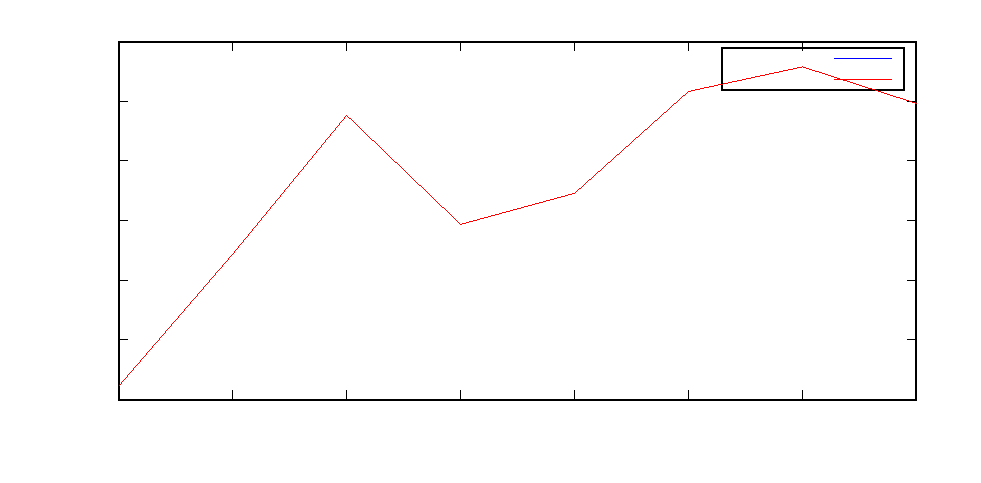
\includegraphics{ej7-grafico-eficiencia-2-cores}}%
    \gplfronttext
  \end{picture}%
\endgroup

	\caption{Tiempos de ejecución mínimos y máximos en 2 cores}
\end{figure}


\subsubsection{3 cores}

\begin{figure}[H]
	\centering
	% GNUPLOT: LaTeX picture with Postscript
\begingroup
  \makeatletter
  \providecommand\color[2][]{%
    \GenericError{(gnuplot) \space\space\space\@spaces}{%
      Package color not loaded in conjunction with
      terminal option `colourtext'%
    }{See the gnuplot documentation for explanation.%
    }{Either use 'blacktext' in gnuplot or load the package
      color.sty in LaTeX.}%
    \renewcommand\color[2][]{}%
  }%
  \providecommand\includegraphics[2][]{%
    \GenericError{(gnuplot) \space\space\space\@spaces}{%
      Package graphicx or graphics not loaded%
    }{See the gnuplot documentation for explanation.%
    }{The gnuplot epslatex terminal needs graphicx.sty or graphics.sty.}%
    \renewcommand\includegraphics[2][]{}%
  }%
  \providecommand\rotatebox[2]{#2}%
  \@ifundefined{ifGPcolor}{%
    \newif\ifGPcolor
    \GPcolorfalse
  }{}%
  \@ifundefined{ifGPblacktext}{%
    \newif\ifGPblacktext
    \GPblacktexttrue
  }{}%
  % define a \g@addto@macro without @ in the name:
  \let\gplgaddtomacro\g@addto@macro
  % define empty templates for all commands taking text:
  \gdef\gplbacktext{}%
  \gdef\gplfronttext{}%
  \makeatother
  \ifGPblacktext
    % no textcolor at all
    \def\colorrgb#1{}%
    \def\colorgray#1{}%
  \else
    % gray or color?
    \ifGPcolor
      \def\colorrgb#1{\color[rgb]{#1}}%
      \def\colorgray#1{\color[gray]{#1}}%
      \expandafter\def\csname LTw\endcsname{\color{white}}%
      \expandafter\def\csname LTb\endcsname{\color{black}}%
      \expandafter\def\csname LTa\endcsname{\color{black}}%
      \expandafter\def\csname LT0\endcsname{\color[rgb]{1,0,0}}%
      \expandafter\def\csname LT1\endcsname{\color[rgb]{0,1,0}}%
      \expandafter\def\csname LT2\endcsname{\color[rgb]{0,0,1}}%
      \expandafter\def\csname LT3\endcsname{\color[rgb]{1,0,1}}%
      \expandafter\def\csname LT4\endcsname{\color[rgb]{0,1,1}}%
      \expandafter\def\csname LT5\endcsname{\color[rgb]{1,1,0}}%
      \expandafter\def\csname LT6\endcsname{\color[rgb]{0,0,0}}%
      \expandafter\def\csname LT7\endcsname{\color[rgb]{1,0.3,0}}%
      \expandafter\def\csname LT8\endcsname{\color[rgb]{0.5,0.5,0.5}}%
    \else
      % gray
      \def\colorrgb#1{\color{black}}%
      \def\colorgray#1{\color[gray]{#1}}%
      \expandafter\def\csname LTw\endcsname{\color{white}}%
      \expandafter\def\csname LTb\endcsname{\color{black}}%
      \expandafter\def\csname LTa\endcsname{\color{black}}%
      \expandafter\def\csname LT0\endcsname{\color{black}}%
      \expandafter\def\csname LT1\endcsname{\color{black}}%
      \expandafter\def\csname LT2\endcsname{\color{black}}%
      \expandafter\def\csname LT3\endcsname{\color{black}}%
      \expandafter\def\csname LT4\endcsname{\color{black}}%
      \expandafter\def\csname LT5\endcsname{\color{black}}%
      \expandafter\def\csname LT6\endcsname{\color{black}}%
      \expandafter\def\csname LT7\endcsname{\color{black}}%
      \expandafter\def\csname LT8\endcsname{\color{black}}%
    \fi
  \fi
  \setlength{\unitlength}{0.0500bp}%
  \begin{picture}(9118.00,4320.00)%
    \gplgaddtomacro\gplbacktext{%
      \colorrgb{0.00,0.00,0.00}%
      \put(740,640){\makebox(0,0)[r]{\strut{}0}}%
      \colorrgb{0.00,0.00,0.00}%
      \put(740,1328){\makebox(0,0)[r]{\strut{}0.2}}%
      \colorrgb{0.00,0.00,0.00}%
      \put(740,2016){\makebox(0,0)[r]{\strut{}0.4}}%
      \colorrgb{0.00,0.00,0.00}%
      \put(740,2703){\makebox(0,0)[r]{\strut{}0.6}}%
      \colorrgb{0.00,0.00,0.00}%
      \put(740,3391){\makebox(0,0)[r]{\strut{}0.8}}%
      \colorrgb{0.00,0.00,0.00}%
      \put(740,4079){\makebox(0,0)[r]{\strut{}1}}%
      \colorrgb{0.00,0.00,0.00}%
      \put(860,440){\makebox(0,0){\strut{}$(1, *, *)$}}%
      \colorrgb{0.00,0.00,0.00}%
      \put(1945,440){\makebox(0,0){\strut{}$(2, *, *)$}}%
      \colorrgb{0.00,0.00,0.00}%
      \put(3031,440){\makebox(0,0){\strut{}$(3, *, *)$}}%
      \colorrgb{0.00,0.00,0.00}%
      \put(4116,440){\makebox(0,0){\strut{}$(4, *, *)$}}%
      \colorrgb{0.00,0.00,0.00}%
      \put(5202,440){\makebox(0,0){\strut{}$(5, *, *)$}}%
      \colorrgb{0.00,0.00,0.00}%
      \put(6287,440){\makebox(0,0){\strut{}$(6, *, *)$}}%
      \colorrgb{0.00,0.00,0.00}%
      \put(7373,440){\makebox(0,0){\strut{}$(7, *, *)$}}%
      \colorrgb{0.00,0.00,0.00}%
      \put(8458,440){\makebox(0,0){\strut{}$(8, *, *)$}}%
      \colorrgb{0.00,0.00,0.00}%
      \put(160,2359){\rotatebox{90}{\makebox(0,0){\strut{}Eficiencia (ciclos \'utiles / ciclos totales)}}}%
      \colorrgb{0.00,0.00,0.00}%
      \put(4659,140){\makebox(0,0){\strut{}Quantums por core}}%
    }%
    \gplgaddtomacro\gplfronttext{%
      \csname LTb\endcsname%
      \put(7555,3916){\makebox(0,0)[r]{\strut{}M\'inimo}}%
      \csname LTb\endcsname%
      \put(7555,3716){\makebox(0,0)[r]{\strut{}M\'aximo}}%
    }%
    \gplbacktext
    \put(0,0){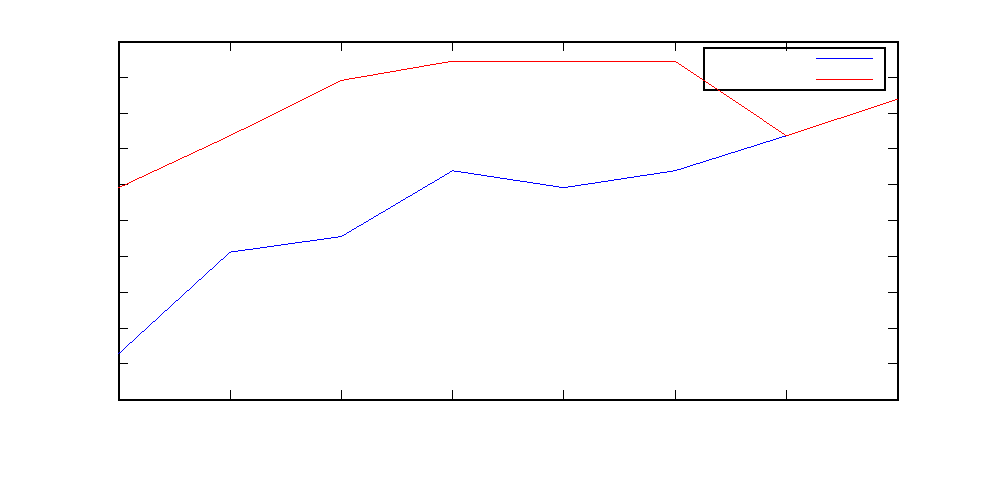
\includegraphics{ej7-grafico-eficiencia-3-cores}}%
    \gplfronttext
  \end{picture}%
\endgroup

	\caption{Tiempos de ejecución mínimos y máximos en 3 cores}
\end{figure}


\subsubsection{4 cores}

\begin{figure}[H]
	\centering
	% GNUPLOT: LaTeX picture with Postscript
\begingroup
  \makeatletter
  \providecommand\color[2][]{%
    \GenericError{(gnuplot) \space\space\space\@spaces}{%
      Package color not loaded in conjunction with
      terminal option `colourtext'%
    }{See the gnuplot documentation for explanation.%
    }{Either use 'blacktext' in gnuplot or load the package
      color.sty in LaTeX.}%
    \renewcommand\color[2][]{}%
  }%
  \providecommand\includegraphics[2][]{%
    \GenericError{(gnuplot) \space\space\space\@spaces}{%
      Package graphicx or graphics not loaded%
    }{See the gnuplot documentation for explanation.%
    }{The gnuplot epslatex terminal needs graphicx.sty or graphics.sty.}%
    \renewcommand\includegraphics[2][]{}%
  }%
  \providecommand\rotatebox[2]{#2}%
  \@ifundefined{ifGPcolor}{%
    \newif\ifGPcolor
    \GPcolorfalse
  }{}%
  \@ifundefined{ifGPblacktext}{%
    \newif\ifGPblacktext
    \GPblacktexttrue
  }{}%
  % define a \g@addto@macro without @ in the name:
  \let\gplgaddtomacro\g@addto@macro
  % define empty templates for all commands taking text:
  \gdef\gplbacktext{}%
  \gdef\gplfronttext{}%
  \makeatother
  \ifGPblacktext
    % no textcolor at all
    \def\colorrgb#1{}%
    \def\colorgray#1{}%
  \else
    % gray or color?
    \ifGPcolor
      \def\colorrgb#1{\color[rgb]{#1}}%
      \def\colorgray#1{\color[gray]{#1}}%
      \expandafter\def\csname LTw\endcsname{\color{white}}%
      \expandafter\def\csname LTb\endcsname{\color{black}}%
      \expandafter\def\csname LTa\endcsname{\color{black}}%
      \expandafter\def\csname LT0\endcsname{\color[rgb]{1,0,0}}%
      \expandafter\def\csname LT1\endcsname{\color[rgb]{0,1,0}}%
      \expandafter\def\csname LT2\endcsname{\color[rgb]{0,0,1}}%
      \expandafter\def\csname LT3\endcsname{\color[rgb]{1,0,1}}%
      \expandafter\def\csname LT4\endcsname{\color[rgb]{0,1,1}}%
      \expandafter\def\csname LT5\endcsname{\color[rgb]{1,1,0}}%
      \expandafter\def\csname LT6\endcsname{\color[rgb]{0,0,0}}%
      \expandafter\def\csname LT7\endcsname{\color[rgb]{1,0.3,0}}%
      \expandafter\def\csname LT8\endcsname{\color[rgb]{0.5,0.5,0.5}}%
    \else
      % gray
      \def\colorrgb#1{\color{black}}%
      \def\colorgray#1{\color[gray]{#1}}%
      \expandafter\def\csname LTw\endcsname{\color{white}}%
      \expandafter\def\csname LTb\endcsname{\color{black}}%
      \expandafter\def\csname LTa\endcsname{\color{black}}%
      \expandafter\def\csname LT0\endcsname{\color{black}}%
      \expandafter\def\csname LT1\endcsname{\color{black}}%
      \expandafter\def\csname LT2\endcsname{\color{black}}%
      \expandafter\def\csname LT3\endcsname{\color{black}}%
      \expandafter\def\csname LT4\endcsname{\color{black}}%
      \expandafter\def\csname LT5\endcsname{\color{black}}%
      \expandafter\def\csname LT6\endcsname{\color{black}}%
      \expandafter\def\csname LT7\endcsname{\color{black}}%
      \expandafter\def\csname LT8\endcsname{\color{black}}%
    \fi
  \fi
  \setlength{\unitlength}{0.0500bp}%
  \begin{picture}(9118.00,4320.00)%
    \gplgaddtomacro\gplbacktext{%
      \colorrgb{0.00,0.00,0.00}%
      \put(860,640){\makebox(0,0)[r]{\strut{}0.36}}%
      \colorrgb{0.00,0.00,0.00}%
      \put(860,1213){\makebox(0,0)[r]{\strut{}0.38}}%
      \colorrgb{0.00,0.00,0.00}%
      \put(860,1786){\makebox(0,0)[r]{\strut{}0.4}}%
      \colorrgb{0.00,0.00,0.00}%
      \put(860,2360){\makebox(0,0)[r]{\strut{}0.42}}%
      \colorrgb{0.00,0.00,0.00}%
      \put(860,2933){\makebox(0,0)[r]{\strut{}0.44}}%
      \colorrgb{0.00,0.00,0.00}%
      \put(860,3506){\makebox(0,0)[r]{\strut{}0.46}}%
      \colorrgb{0.00,0.00,0.00}%
      \put(860,4079){\makebox(0,0)[r]{\strut{}0.48}}%
      \colorrgb{0.00,0.00,0.00}%
      \put(980,440){\makebox(0,0){\strut{}$(1, *, *, *)$}}%
      \colorrgb{0.00,0.00,0.00}%
      \put(2023,440){\makebox(0,0){\strut{}$(2, *, *, *)$}}%
      \colorrgb{0.00,0.00,0.00}%
      \put(3065,440){\makebox(0,0){\strut{}$(3, *, *, *)$}}%
      \colorrgb{0.00,0.00,0.00}%
      \put(4108,440){\makebox(0,0){\strut{}$(4, *, *, *)$}}%
      \colorrgb{0.00,0.00,0.00}%
      \put(5150,440){\makebox(0,0){\strut{}$(5, *, *, *)$}}%
      \colorrgb{0.00,0.00,0.00}%
      \put(6193,440){\makebox(0,0){\strut{}$(6, *, *, *)$}}%
      \colorrgb{0.00,0.00,0.00}%
      \put(7235,440){\makebox(0,0){\strut{}$(7, *, *, *)$}}%
      \colorrgb{0.00,0.00,0.00}%
      \put(8278,440){\makebox(0,0){\strut{}$(8, *, *, *)$}}%
      \colorrgb{0.00,0.00,0.00}%
      \put(160,2359){\rotatebox{90}{\makebox(0,0){\strut{}Eficiencia (ciclos \'utiles / ciclos totales)}}}%
      \colorrgb{0.00,0.00,0.00}%
      \put(4629,140){\makebox(0,0){\strut{}Quantums por core}}%
    }%
    \gplgaddtomacro\gplfronttext{%
      \csname LTb\endcsname%
      \put(7375,3916){\makebox(0,0)[r]{\strut{}M\'inimo}}%
      \csname LTb\endcsname%
      \put(7375,3716){\makebox(0,0)[r]{\strut{}M\'aximo}}%
    }%
    \gplbacktext
    \put(0,0){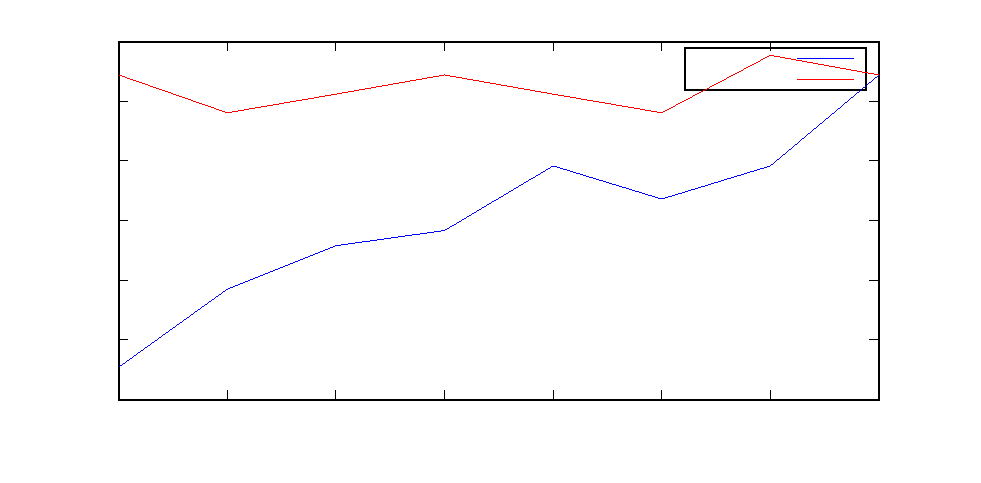
\includegraphics{ej7-grafico-eficiencia-4-cores}}%
    \gplfronttext
  \end{picture}%
\endgroup

	\caption{Tiempos de ejecución mínimos y máximos en 4 cores}
\end{figure}


\subsection{Resultados}

Los resultados a continuación son las configuraciones óptimas de quantums por cantidad de cores para cada métrica. Estas configuraciones óptimas no siempre son únicas. En caso de haber más de una, se muestra la que primero se alcanza realizando los experimentos en la secuencia descrita en la sección anterior.

Recordar que estas configuraciones son óptimas \textbf{sólo para el lote de tareas estudiado}. Para lotes distintos estos valores podrían ser subóptimos.


\subsubsection{Tiempo de ejecución}

\begin{description}
	\item[1 core:] $1$.             Tiempo demorado: 224 ticks.
	\item[2 cores:] $(7, 7)$.       Tiempo demorado: 126 ticks.
	\item[3 cores:] $(3, 7, 7)$.    Tiempo demorado: 91 ticks.
	\item[4 cores:] $(7, 8, 8, 8)$. Tiempo demorado: 70 ticks.
\end{description}


\subsubsection{Eficiencia}

\begin{description}
	\item[1 core:] $1$.             Eficiencia alcanzada: 60\%.
	\item[2 cores:] $(7, 7)$.       Eficiencia alcanzada: 53.15\%.
	\item[3 cores:] $(4, 8, 8)$.    Eficiencia alcanzada: 49.45\%.
	\item[4 cores:] $(7, 8, 8, 8)$. Eficiencia alcanzada: 47.53\%.
\end{description}


%%%%%%%%%%%%%%%%%%%%%%%%%%%%%%%%%%%%%%%%%%%%%%%%%%%%%%%%%%%%%%%%%%%%%%%%%%%%%%%
%% Ejercicio 8                                                               %%
%%%%%%%%%%%%%%%%%%%%%%%%%%%%%%%%%%%%%%%%%%%%%%%%%%%%%%%%%%%%%%%%%%%%%%%%%%%%%%%


\section{Ejercicio 8}

\subsection{Medición e hipótesis}
Consideramos como unidad de medición los ticks realizados por los procesadores para un lote de tareas. Esta elección se debe a que, para nuestro criterio, un scheduler tiene una mejor pérformance (se desempeña mejor), si logra terminar el lote de tareas en menos tiempo (ticks) que otro.

Analizando los dos algoritmos, deducimos dos hipótesis que muestran los beneficios y los contra que poseen ambos algoritmos.

La primera hipótesis es que, el algoritmo de SchedRR presentaría tiempos sin uso del procesador debido a la penalidad de cambio de nucleos, mientras que el algoritmo de SchedRR2 no los tendría debido a que este no lo permite, haciendo que necesite más ticks para completar el lote de tareas.

Como segunda hipótesis, teniendo una penalidad baja para migrar tareas de un core a otro,  el algoritmo SchedRR se comportaría mejor que SchedRR2 debido a que al algoritmo SchedRR2 no le es posible migrar procesos, interrumpiendo en alguna medida el paralelismo otorgado por tener múltiples cores.

\subsection{Experimentos}

Para realizar el experimento del mal funcionamiento del SchedRR utilizando alta penalidad, se consiguieron 400 tiempos promedios de ejecución. Estos tiempos promedios se calcularon como la suma de la cantidad de ticks utilizados de 50 lotes de tareas dividido 50. Se utilizaron 2 cores de quantum 100 en ambos y 4 tareas \textit{RandomTask} las cuales tienen bloqueos y consumos de CPU aleatorios (utilizando una seed para realizar el mismo experimento en ambos schedulers) en duración y en cantidad. En cada uno de los 400 promedios, se incrementó en ambos la penalidad de core switch.

\begin{figure}[ht!]
\centering
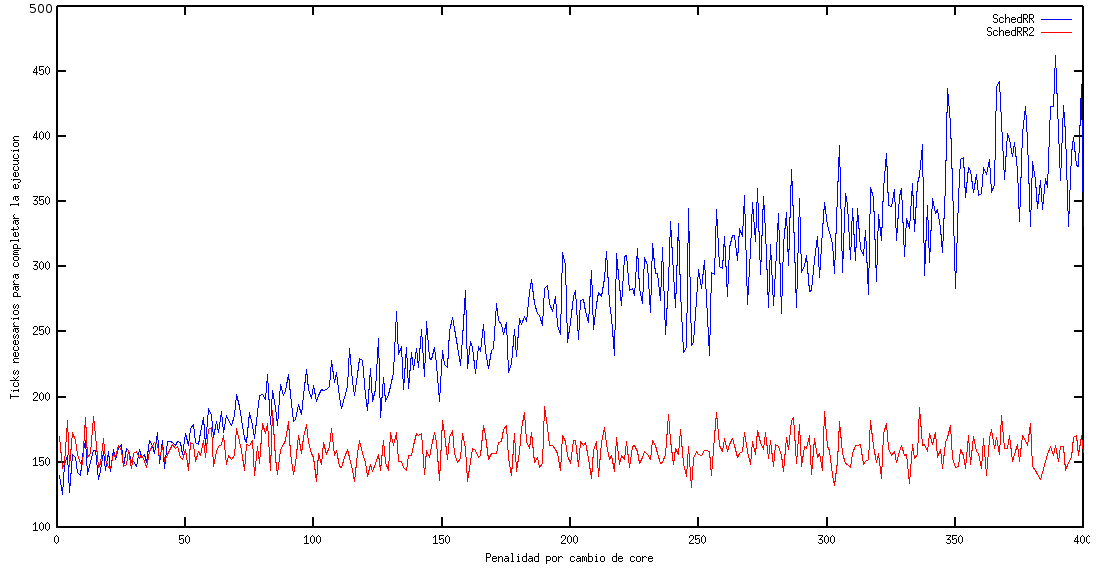
\includegraphics[width=175mm]{../ejercicio8/compTicksSched.png}
\caption{Comparación de ticks necesarios para ambos schedulers}
\label{overflow}
\end{figure}

Como puede observarse en la figura 7, a partir de una penalidad de 50, el SchedRR empieza a necesitar más ticks para completar las tareas que el SchedRR2, haciendo del SchedRR2 una mejor opción para el caso de penalidades altas. Sin embargo, de 50 ticks para abajo, el SchedRR realiza un mejor trabajo, terminando la ejecución del lote de tareas más rápido que el SchedRR2.

En igualdad de condiciones, realizando otra vez un test aleatorio, de iguales condiciones que el experimento anterior, esta vez sin incrementar el costo de migración, se obtiene la figura 11. Esta figura, muestra de a pares (ticks necesarios utilizando ScheddRR y ticks necesarios con SchedRR2), un subconjunto del experimento realizado en el cual se puede ver que en la mayoría de los casos, SchedRR2 supera al SchedRR en ticks para completar el lote de tareas.

Para una mejor apreciación global, se presenta la siguiente tabla: \\
\\
\begin{tabular}{| l | c |}
  \hline                        
  Experimentos donde SchedRR tarda hasta $10\%$ menos ticks que SchedRR2 & 341 \\
  Experimentos donde SchedRR tarda más de $10\%$ menos ticks que SchedRR2 & 3 \\
  Experimentos donde SchedRR2 tarda hasta $10\%$ menos que SchedRR2 & 56 \\
  \hline  
\end{tabular}

\begin{figure}[ht!]
\centering
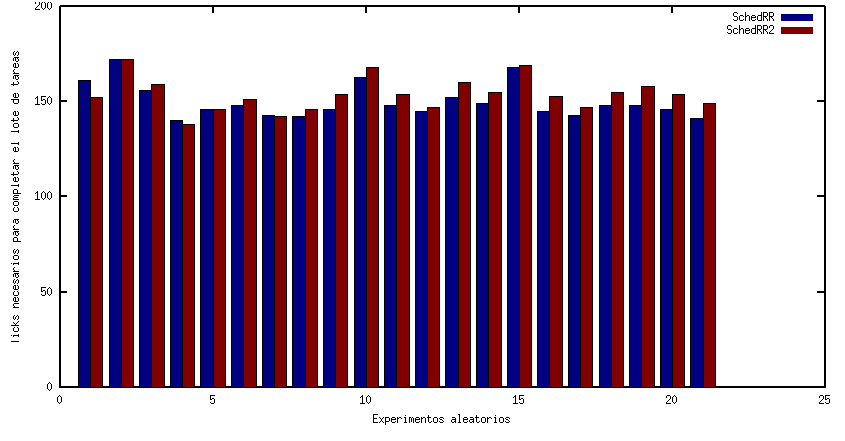
\includegraphics[width=175mm]{../ejercicio8/comTicksSchedIgualdad.png}
\caption{Comparación de ticks necesarios para ambos schedulers con igualdad de parámetros}
\label{overflow}
\end{figure}

Se puede notar, como en la mayoría de los casos, en igualdad de condiciones y para costos de migración bajos, el SchedRR tarda menos que el SchedRR2 en ejecutar un lote de tareas.

Esto se debe a que el algoritmo de SchedRR al tener una única cola de procesos, puede asignar siempre una tarea a un core libre, mientras que en SchedRR2, uno de los cores puede haber terminado de ejecutar su cola de tareas más rápido que el otro core, quedando este sin utilizarse.

\begin{figure}[ht!]
\centering
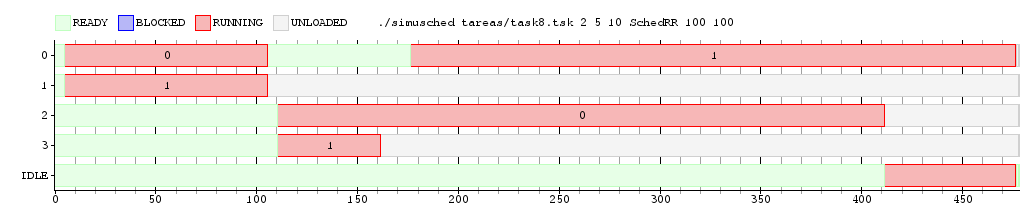
\includegraphics[width=175mm]{../ejercicio8/schedRRej8.png}
\caption{Ejecución de lote de tareas utilizando SchedRR}
\label{overflow}
\end{figure}

\begin{figure}[ht!]
\centering
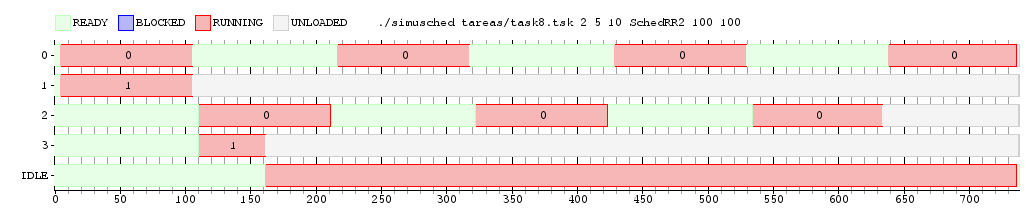
\includegraphics[width=175mm]{../ejercicio8/schedRR2ej8.png}
\caption{Ejecución de lote de tareas utilizando SchedRR2}
\label{overflow}
\end{figure}

Puede notarse la diferencia mencionada en la figura 9 y la figura 10. En la figura 9, relacionada al SchedRR, cuándo el core 1 termina de ejecutar la tarea 3, pasa a ejecutar la tarea 0, dejando que el core 0 se encargue de la ejecución de la tarea 2. Por el contrario, en la figura 10, al terminar el core 1 la ejecución de la tarea 3, este queda sin utilizarse, dejandole la tarea de la ejecución de las tareas 0 y 2 únicamente al core 0 el cuál, sin el core 1, necesita más ticks para completar estas tareas.

%%%%%%%%%%%%%%%%%%%%%%%%%%%%%%%%%%%%%%%%%%%%%%%%%%%%%%%%%%%%%%%%%%%%%%%%%%%%%%%
%% Ejercicio 9                                                               %%
%%%%%%%%%%%%%%%%%%%%%%%%%%%%%%%%%%%%%%%%%%%%%%%%%%%%%%%%%%%%%%%%%%%%%%%%%%%%%%%


\section{Ejercicio 9}

Pendiente.


%%%%%%%%%%%%%%%%%%%%%%%%%%%%%%%%%%%%%%%%%%%%%%%%%%%%%%%%%%%%%%%%%%%%%%%%%%%%%%%
%% Ejercicio 10                                                              %%
%%%%%%%%%%%%%%%%%%%%%%%%%%%%%%%%%%%%%%%%%%%%%%%%%%%%%%%%%%%%%%%%%%%%%%%%%%%%%%%


\section{Ejercicio 10}

Pendiente.


%%%%%%%%%%%%%%%%%%%%%%%%%%%%%%%%%%%%%%%%%%%%%%%%%%%%%%%%%%%%%%%%%%%%%%%%%%%%%%%
%% Conclusiones                                                              %%
%%%%%%%%%%%%%%%%%%%%%%%%%%%%%%%%%%%%%%%%%%%%%%%%%%%%%%%%%%%%%%%%%%%%%%%%%%%%%%%


\section{Conclusiones}

Pendiente.


%%%%%%%%%%%%%%%%%%%%%%%%%%%%%%%%%%%%%%%%%%%%%%%%%%%%%%%%%%%%%%%%%%%%%%%%%%%%%%%
%% Apéndice                                                                  %%
%%%%%%%%%%%%%%%%%%%%%%%%%%%%%%%%%%%%%%%%%%%%%%%%%%%%%%%%%%%%%%%%%%%%%%%%%%%%%%%

\newpage

\begin{appendices}

\section{Apéndice}

Pendiente.


\end{appendices}

\end{document}